%!TEX TS-program = xelatex 
%!TEX TS-options = -output-driver="xdvipdfmx -q -E"
%!TEX encoding = UTF-8 Unicode
%
%  my_title
%
%  Created by my_name on date.
%  Copyright (c) year. All rights reserved.
%

\documentclass[12pt]{article} 

% Definitions
\newcommand\mykeywords{color, illusion} 
\newcommand\myauthor{Mark Eli Kallderon} 
\newcommand\mytitle{Color Illusion}
\newcommand\mybib{Philosophy.bib}

% Packages
\usepackage{geometry} \geometry{a4paper} 
\usepackage{url}
\usepackage{txfonts}
\usepackage{color}
\definecolor{gray}{rgb}{0.459,0.438,0.471}
% \usepackage{setspace}
% \doublespace % Uncomment for doublespacing if necessary
\usepackage{epigraph} % optional

% XeTeX
\usepackage[cm-default]{fontspec}
\usepackage{xltxtra,xunicode}
\defaultfontfeatures{Scale=MatchLowercase,Mapping=tex-text}
\setmainfont{Palatino}
\setsansfont{Gill Sans}
\setmonofont{Inconsolata}

% Section Formatting
\usepackage[]{titlesec}
\titleformat{\section}[hang]{\fontsize{14}{14}\scshape}{\S{\thesection}}{.5em}{}{}
\titleformat{\subsection}[hang]{\fontsize{12}{12}\scshape}{\S{\thesubsection}}{.5em}{}{}
\titleformat{\subsubsection}[hang]{\fontsize{12}{12}\scshape}{\S{\thesubsubsection}}{.5em}{}{}

% Headers and Footers
\usepackage{fancyhdr}
\pagestyle{fancy}
\pagenumbering{arabic}
\lhead{\thepage}
\chead{}
\rhead{\itshape{\nouppercase{\leftmark}}}

% TODO List
\usepackage{color}
\usepackage{index} % use index package to create indices
\newindex{todo}{tod}{tnd}{TODO List} % start todo list
\newindex{fixme}{fix}{fnd}{FIXME List} % start fixme list
\newcommand{\todo}[1]{\textcolor{blue}{TODO: #1}\index[todo]{#1}} % macro for todo entries
\newcommand{\fixme}[1]{\textcolor{red}{FIXME: #1}\index[fixme]{#1}} % macro for fixme entries

% Bibliography
\usepackage[round]{natbib} 

% Title Information
\title{\mytitle} % For thanks comment this line and uncomment the line below
%\title{\mytitle\thanks{}}% 
\author{\myauthor} 
% \date{} % Leave blank for no date, comment out for most recent date

% PDF Stuff
\usepackage[plainpages=false, pdfpagelabels, bookmarksnumbered, backref, pdftitle={\mytitle}, pagebackref, pdfauthor={\myauthor}, pdfkeywords={\mykeywords}, xetex, dvipdfmx, colorlinks=true, citecolor=gray, linkcolor=gray, urlcolor=gray]{hyperref} 



%%% BEGIN DOCUMENT
\begin{document}

% Title Page
\maketitle
% \begin{abstract} % optional
% \end{abstract} 
\vskip 2em \hrule height 0.4pt \vskip 2em
% \epigraph{text of epigraph}{\textsc{author of epigraph}} % optional; make sure to uncomment \usepackage{epigraph}

% Layout Settings
\setlength{\parindent}{1em}

% Main Content

\section{Introduction} % (fold)
\label{sec:introduction}

I have lost my grip on what a color illusion is meant to be. Perhaps I have simply lost my grip---not an alternative to be ruled out in advance of inquiry. However, I believe that there is an alternative explanation. I have come to suspect that there is nothing answering to the philosopher's conception of illusion. That's not to say that there are no color experiences that might, with propriety, be described as illusory. There is a familiar genre of books illustrating optical illusions, many essentially involving chromatic phenomena. No charge of false advertising is leveled here. It is only a distinctively philosophical conception of illusion whose claims are exaggerated. Or so I have, lately, come to suspect.

% section introduction (end)

\section{Benham's Disk} % (fold)
\label{sec:benham_s_disk}

Let's begin by considering an example of a color illusion often cited by philosophers---Benahma's disk.

In 1894, an English toymaker, Charles Benham, devised a top adorned with a black and white pattern (see Figure~\ref{fig:benham}). Sold through Messrs. Newton and Co., an announcement of the ``Artifical Spectrum Top'' was published in \emph{Nature}:
\begin{quote}
	The top consists of a disc, one half of which is black, while the other half has twelve arcs of concentric circles drawn upon it. Each arc subtends an angle of forty-five degrees. In the first quadrant there are three such concentric arcs, in the next three more, and so on ; the only difference being that the arcs are parts of circles of which the radii increase in arithmetical progression. Each quadrant thus contains a group of arcs differing in length from those of the other quadrants. The curious point is that when this disc is revolved, the impression of concentric circles of different colors is produced upon the retina. If the direction of rotation is reversed, the order of these tints is also reversed. \citep{Benham:1894kx}
\end{quote}
Specifically, if rotated clockwise, the innermost arcs form reddish rings, the next greenish rings, the next light blue rings, and the outermost arcs form violet rings. If rotated counterclockwise the pattern is reversed with the innermost arcs now forming violet rings and the outermost reddish rings. These apparent colors are puzzling. Each of the spinning arcs reflect light of with the same spectral content and with equal average luminance. In advance of observing the spinning disk, then, one might reasonably expect the spinning arcs to appear as gray rings of equal brightness. The mysterious apparent colors of Benham's spinning disk are the ``subjective colors'' first described by \citep{Fechner:1838vn} (and, hence, are also sometimes described as ``Fechner-Benham colors'', also, variously, ``polyphän'' colors and ``pattern-induced flicker colors'' or PIFCs). The subjective colors produced by Benham's spinning disk are not completely understood. For a review of some of the color science see \citet{Campenhausen:1995yq}.

\begin{figure}[htbp]
	\centering
		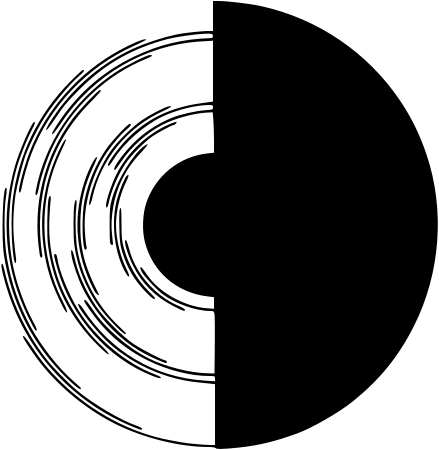
\includegraphics[scale=.5]{graphics/benhams_disk.jpg}
	\caption{Benham's Disk}
	\label{fig:benham}
\end{figure}



% section benham_s_disk (end)

% Bibligography
\bibliographystyle{plainnat} 
\bibliography{Philosophy.bib} 

\end{document}
